\documentclass{beamer}
\mode<presentation>
\usepackage{amsmath}
\usepackage{amssymb}
%\usepackage{advdate}
\usepackage{adjustbox}
\usepackage{subcaption}
\usepackage{enumitem}
\usepackage{multicol}
\usepackage{mathtools}
\usepackage{listings}
\usepackage{url}
\def\UrlBreaks{\do\/\do-}
\usetheme{Boadilla}
\usecolortheme{lily}
\setbeamertemplate{footline}
{
  \leavevmode%
  \hbox{%
  \begin{beamercolorbox}[wd=\paperwidth,ht=2.25ex,dp=1ex,right]{author in head/foot}%
    \insertframenumber{} / \inserttotalframenumber\hspace*{2ex} 
  \end{beamercolorbox}}%
  \vskip0pt%
}
\setbeamertemplate{navigation symbols}{}

\providecommand{\nCr}[2]{\,^{#1}C_{#2}} % nCr
\providecommand{\nPr}[2]{\,^{#1}P_{#2}} % nPr
\providecommand{\mbf}{\mathbf}
\providecommand{\pr}[1]{\ensuremath{\Pr\left(#1\right)}}
\providecommand{\qfunc}[1]{\ensuremath{Q\left(#1\right)}}
\providecommand{\sbrak}[1]{\ensuremath{{}\left[#1\right]}}
\providecommand{\lsbrak}[1]{\ensuremath{{}\left[#1\right.}}
\providecommand{\rsbrak}[1]{\ensuremath{{}\left.#1\right]}}
\providecommand{\brak}[1]{\ensuremath{\left(#1\right)}}
\providecommand{\lbrak}[1]{\ensuremath{\left(#1\right.}}
\providecommand{\rbrak}[1]{\ensuremath{\left.#1\right)}}
\providecommand{\cbrak}[1]{\ensuremath{\left\{#1\right\}}}
\providecommand{\lcbrak}[1]{\ensuremath{\left\{#1\right.}}
\providecommand{\rcbrak}[1]{\ensuremath{\left.#1\right\}}}
\theoremstyle{remark}
\newtheorem{rem}{Remark}
\newcommand{\sgn}{\mathop{\mathrm{sgn}}}
\providecommand{\abs}[1]{\left\vert#1\right\vert}
\providecommand{\res}[1]{\Res\displaylimits_{#1}} 
\providecommand{\norm}[1]{\lVert#1\rVert}
\providecommand{\mtx}[1]{\mathbf{#1}}
\providecommand{\mean}[1]{E\left[ #1 \right]}
\providecommand{\fourier}{\overset{\mathcal{F}}{ \rightleftharpoons}}
%\providecommand{\hilbert}{\overset{\mathcal{H}}{ \rightleftharpoons}}
\providecommand{\system}{\overset{\mathcal{H}}{ \longleftrightarrow}}
	%\newcommand{\solution}[2]{\textbf{Solution:}{#1}}
%\newcommand{\solution}{\noindent \textbf{Solution: }}
\providecommand{\dec}[2]{\ensuremath{\overset{#1}{\underset{#2}{\gtrless}}}}
\newcommand{\myvec}[1]{\ensuremath{\begin{pmatrix}#1\end{pmatrix}}}
\let\vec\mathbf

\lstset{
language=C,
frame=single, 
breaklines=true,
columns=fullflexible
}

\numberwithin{equation}{section}

\title{Presentation - Matgeo}
\author{Satyanarayana Gajjarapu \\
AI24BTECH11009 \\
EE1030 - Matrix Theory}

\date{\today} 
\begin{document}

\begin{frame}
\titlepage
\end{frame}

\section*{Outline}
\begin{frame}
\tableofcontents
\end{frame}
\section{Problem}
\begin{frame}
\frametitle{Problem Statement}
If the lines $2x - 3y = 5$ and $3x - 4y = 7$ are the diameters of a circle of area 154 square units, then obtain the equation of the circle.
\end{frame}

%\subsection{Literature}
\section{Solution}
\subsection{Description of Variables used}
\begin{frame}
\frametitle{Description of Variables used}
    \begin{table}[h!]
  \centering
  \begin{tabular}[12pt]{ |c| c|}
    \hline
    \textbf{Variables} & \textbf{Description}\\ 
    \hline
    $\textbf{V}_1, \vec{u}_1, f_1$ & Parameters of the parabola $y^2 = 4x$ \\
    \hline
     $\textbf{V}_2, \vec{u}_2, f_2$ & Parameters of the circle $4x^2 + 4xy^2 = 9$ \\
    \hline
    $\vec{x}^\intercal\brak{\textbf{V}_1 + \mu\textbf{V}_2}\vec{x} + 2\brak{\vec{u}_1 + \mu\vec{u}_2}^\intercal\vec{x} + \brak{f_1 + \mu f_2}$ & Intersection of two conics \\
    \hline
    \end{tabular}


\end{table}
\end{frame}
\subsection{Row Reduction: Finding $\vec{c}$}
\begin{frame}
\frametitle{Row Reduction: Finding $\vec{c}$}
The augmented matrix formed by the given equations of diameter is
\begin{align}
    \myvec{2 & -3 & 5 \\ 3 & -4 & 7} \xrightarrow[]{R_2 \rightarrow 2R_2 - 3R_1} & \myvec{2 & -3 & 5 \\ 0 & 1 & -1} \\
    \xrightarrow[]{R_1 \rightarrow R_1 + 3R_2} & \myvec{2 & 0 & 2 \\ 0 & 1 & -1} \\
    \xrightarrow[]{R_1 \rightarrow \frac{R_1}{2}} & \myvec{1 & 0 & 1 \\ 0 & 1 & -1} \label{eq7.2.23.1}
\end{align}
Therefore from equation \ref{eq7.2.23.1}
\begin{align}
    \vec{c} & = \myvec{1 \\ -1}
\end{align}
\end{frame}
\subsection{Finding $\vec{u}$, $r$ and $f$}
\begin{frame}
\frametitle{Finding $\vec{u}$, $r$ and $f$}
\begin{align}
    \vec{u} & = \myvec{-1 \\ 1} \\
    \vec{u}^\intercal & = \myvec{-1 & 1} \\
    \lVert\vec{u}\rVert^2 & = \vec{u}^\intercal \vec{u} \\
    \lVert\vec{u}\rVert^2 & = 2
    \end{align}
    Given area is 154 square units
\begin{align}
    \pi r^2 & = 154 \\
    r & = 7 \\
    f & = 2 - 49 \\
    f & = -47
\end{align}
\end{frame}
%\section{Plot}
\subsection{Equation of Circle}
\begin{frame}
\frametitle{Equation of Circle}
The equation of circle is given by
\begin{align}
    \lVert\vec{x}\rVert^2 + 2\vec{u}^\intercal\vec{x} + f & = 0 \\
    \vec{x}^\intercal\vec{x} + 2\myvec{-1 & 1}\vec{x} + (-47) & = 0 \\
    x^2 + y^2 - 2x + 2y - 47 & = 0 \label{eq:circ_eq}
\end{align}
\end{frame}
\subsection{Plot}
\begin{frame}
    \frametitle{Plot}
\begin{figure}[h!]
   \centering
   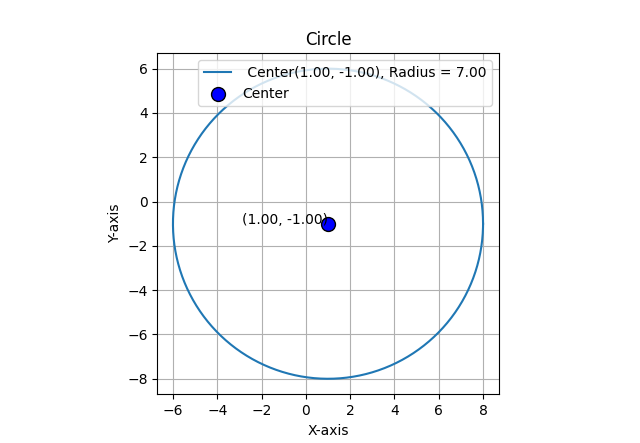
\includegraphics[width=0.9\linewidth]{figs/circle.png}
   \end{figure}
\end{frame}
\subsection{Codes}
\begin{frame}[fragile]
    \frametitle{Code - C}
    The code to find the equation of circle is
    \begin{lstlisting}
#include <stdio.h>
#include <math.h>

#define NUM_POINTS 500

void findCenter(float a1, float b1, float c1, float a2, float b2, float c2, float* centerX, float* centerY) {
    float determinant = a1 * b2 - a2 * b1;
    if (determinant != 0) {
        *centerX = (b1 * c2 - b2 * c1) / determinant;
        *centerY = (a2 * c1 - a1 * c2) / determinant;
    } else {
        printf("The lines are parallel, no intersection found.\n");
    }
    }

\end{lstlisting}
\end{frame}
\begin{frame}[fragile]
    \frametitle{Code - C}
    \begin{lstlisting}
    float calculateRadius(float area) {
    float pi = 22.0 / 7.0;
    return sqrt(area / pi);
}
    int main() {
    float a1 = 2, b1 = -3, c1 = -5;   
    float a2 = 3, b2 = -4, c2 = -7;   
    float area = 154.0;               
    float centerX, centerY, radius;
    findCenter(a1, b1, c1, a2, b2, c2, &centerX, &centerY);
    radius = calculateRadius(area);

    printf("Center of the circle: (%.2f, %.2f)\n", centerX, centerY);
    printf("Radius of the circle: %.2f\n", radius);
     printf("Equation of the circle: (x - (%.2f))^2 + (y - (%.2f))^2 = %.2f\n", centerX, centerY, radius * radius);
    \end{lstlisting}
\end{frame}
\begin{frame}[fragile]
    \frametitle{Code - C}
    \begin{lstlisting}
     FILE *file = fopen("coordinates.txt", "w");
    if (file == NULL) {
        printf("Error opening file!\n");
        return 1;
    }
    for (int i = 0; i < NUM_POINTS; i++) {
        float theta = (2 * M_PI * i) / NUM_POINTS; // Angle in radians
        float x = centerX + radius * cos(theta);
        float y = centerY + radius * sin(theta);
        fprintf(file, "%.4f, %.4f\n", x, y);
    }

    fclose(file);
    return 0;
}
    \end{lstlisting}
\end{frame}
\begin{frame}[fragile]
    \frametitle{Code - Python}
    The code to obtain the required plot is
    \begin{lstlisting}
from ctypes import *
import numpy as np
import matplotlib.pyplot as plt
circle_lib = CDLL('./circle.so')
circle_lib.findCenter.argtypes = [c_float, c_float, c_float, c_float, c_float,                                                       c_float, POINTER(c_float), POINTER(c_float)]
circle_lib.calculateRadius.argtypes = [c_float]
circle_lib.calculateRadius.restype = c_float
a1, b1, c1 = 2.0, -3.0, -5.0  
a2, b2, c2 = 3.0, -4.0, -7.0  
area = 154.0  
centerX = c_float(0)
centerY = c_float(0)
circle_lib.findCenter(a1, b1, c1, a2, b2, c2, byref(centerX), byref(centerY))
centerX = centerX.value
\end{lstlisting}
\end{frame}
\begin{frame}[fragile]
    \frametitle{Code - Python}
\begin{lstlisting}
centerY = centerY.value 
radius = circle_lib.calculateRadius(area)
points = np.loadtxt("coordinates.txt", delimiter=",", unpack=False)
plt.figure()
plt.plot(points[:, 0], points[:, 1], color='green', label=f"Circle")
plt.scatter(centerX, centerY, color='blue', s=100, label="Center", edgecolor='black')  
plt.text(centerX, centerY, f"({centerX:.2f}, {centerY:.2f})", fontsize=10, ha='right', color='black')
plt.xlabel("X-axis")
plt.ylabel("Y-axis")
plt.title("Circle")
plt.legend(loc='upper right')
plt.gca().set_aspect('equal', adjustable='box')
plt.grid(True)
plt.show()
    \end{lstlisting}
    \end{frame}
\end{document}

